%&pdflatex
\documentclass[12pt,a4paper]{article}
\usepackage[left=1in,right=1in, bottom=1in]{geometry}
\usepackage[utf8]{inputenc}
\usepackage[english]{babel}			%other options: frenchb,german
\usepackage[pdftex]{graphicx}
\usepackage{moreverb}
\usepackage[hidelinks]{hyperref}
\usepackage{titling}
\usepackage{caption}
\usepackage{listings}

% move title to top of page
\setlength{\droptitle}{-10em}

% remove additional space between tables and their captions
\captionsetup[table]{skip=0pt}
\graphicspath{{figures/}}

% title setup
\title{Robotics Challenge 2015}
\date{May 28, 2015}
\author{
	Fabienne \textsc{Guertler}\\
	IN.2022 Robotics, BSc Course, 2nd Sem.\\
	University of Fribourg \\
	\href{mailto:fabienne.guertler@unifr.ch}{fabienne.guertler@unifr.ch}
}

% setup page
\sloppy
\pagenumbering{roman}
\pagestyle{plain}
\pagenumbering{arabic}
\pagestyle{headings}

\begin{document}
%################### Report Start #####################################
\maketitle

\begin{abstract}
\noindent Brief description of the content (5-10 lines). Helps people decide whether the report is relevant for them or not. Usually written at the end.
\end{abstract}
~~~\indent \textbf{Keywords.} add, keywords, for, indexing

\section*{Introduction}
Objectives of this project and brief description of the problem at hand, the achieved solution and results.

\section{Problem statement}
%Description of the challenge and the environment (e-puck robots, ASEBA suite, and lab).
There are 3 e-pucks in an arena. In this arena there are 2 blue doors and 4 red switches. To open a door a switch must be pressed, meaning to pass through a door two e-pucks have to work together. One finds either the door or the switch and waits in front of it while the other searches the missing component. Once both the door and the switch have been found the door opens and the e-puck can pass. Another requirement for the challenge is that all e-pucks must have the same code, except for calibration values. Before I begin presenting one of the many possible solution strategies I'll present the e-puck and the arena in detail.

\paragraph{E-puck}
The Ecole Polytechnique Fédérale de Lausanne started the e-puck project with the main goal to develop a miniature mobile robot for educational purposes. 
\begin{figure}[h!]
\begin{center}
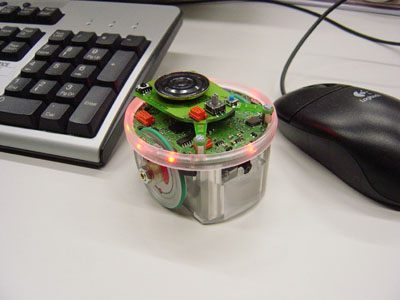
\includegraphics[width = 5cm]{images/epuck-look.jpg}
\caption{E-puck}
\label{fig:epuck}
\end{center}
\end{figure}

The design of the e-puck is based on desktop size and flexibility. By default it comes with sound sensors, a 3D accelerometer, 8 proximity sensors and a camera. It is possible to extend the e-puck with more hardware like a Color LED Communication Turret, groundsensors, magnetic wheels and more.

\begin{figure}[h!]
\begin{center}
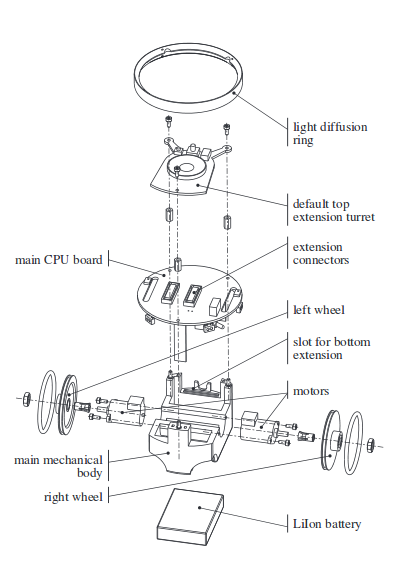
\includegraphics[scale=0.5]{images/epuck-concept.png}
\caption{Mechanical structure}
\label{fig:epuck structure}
\end{center}
\end{figure} 
The structure is based on one single part to keep the desing simple and elegant. This basic part has a diameter of 7 cm and supports the motor, the circuit and the battery. The e-puck uses a miniature stepper motor with gear reduction and the wheels have a diameter of 4,1 cm.

\section{Solution Strategy} \label{sec:solStrategy}
Description of the approach chosen to solve the challenge.

\section{Implementation}
Description of how the solution strategy in Section \ref{sec:solStrategy} was implemented. Only short excerpts of code or pseudo code should be used here. Longer excerpts can be included in \ref{app:sourceCode}.

\section{Validation}
Description of how the solution turned out and what problems were encountered. Since this report is accompanied by a short video, it can be referenced to illustrate the result.

\section*{Conclusion}
Synthesis of the paper and outlook for further work.

\section*{Personal Comments}
Feedback to the course and project (what you liked, what you didn't like, what you learned, ...).

%------------------- Bibliography Start -------------------------------
\begin{thebibliography}{20}
\bibitem{Writing}
Justin Zobel.											% author
\textit{Writing for Computer Science}, 2nd edition.		% title (italics), edition
Springer-Verlag, London, 2004, 275 pages.				% editor, date, other info

% book source
\bibitem{Braitenberg} % cited with '\cite{Braitenberg}'
Valentino Braitenberg.									% author (Firstname Lastname, Firstname2 Lastname2, ...)
\textit{Vehicles: Experiments in Synthetic Psychology}.	% title (italics)
MIT Press, 1986.										% editor, date

% web source
\bibitem{AsebaManual} % cited with '\cite{AsebaManual}'
														% author (sometimes not available)
\textit{Aseba User Manual}.										% title (italics)
https://aseba.wikidot.com/en:asebausermanual.			% url
Last visited: 29.04.15.									% date
\end{thebibliography}
%------------------- Bibliography End -------------------------------
%################### Report End #####################################
%################### Appendix Start #####################################
\appendix
\renewcommand{\thesection}{Appendix \Alph{section}}
\renewcommand{\thesubsection}{\Alph{section}.\arabic{subsection}}

\clearpage

\section{Experimental Results}
Place to list the gathered data.

\section{Source Code} \label{app:sourceCode}
Place to list source code.

\subsection{Advanced Love Behavior} \label{app:advLove} % referenced with '\ref{app:code}'
The code below shows an e-puck implementing the advanced love behavior.
\lstinputlisting[basicstyle=\ttfamily, frame=single, tabsize=4, numbers=left, firstline=29, lastline=57]{code/code.aesl}


\subsection{Explore Behavior} \label{app:expl} % referenced with '\ref{app:code}'
The code below shows an e-puck implementing the explore behavior.
\lstinputlisting[basicstyle=\ttfamily, frame=single, tabsize=4, numbers=left, firstline=60, lastline=88]{code/code.aesl}

%------------------- TODO: Remove Examples Start -------------------------------
\section{\LaTeX{} Examples} % only for demonstration, remove this section
This section shows some common uses of \LaTeX{} features.
\subsection{Images}
Example of how to include an image can be seen in Figure \ref{fig:graphicfile}. All figures must be referenced somewhere in the report.
\begin{figure}[htb]
\begin{center}

\includegraphics[width=7cm]{garfield}
\caption{Including an image.}
\label{fig:graphicfile} % no file ending
\end{center}
\end{figure}

\subsection{Tables}
Example of how to include a table can be seen in Figure \ref{fig:someTable}. All figures must be referenced somewhere in the report.
\begin{figure}[h]
\begin{center}
\begin{tabular}{|c|c|}
\hline
\textbf{Title 1} & \textbf{Title 2} \\
\hline
item 11	&	item 12	\\
\hline
item 21	&	item 22	\\
\hline
\end{tabular}
\end{center}
\caption{Table with caption.}
\label{fig:someTable}
\end{figure}

\subsection{Listings}
Example of how to include listing can be seen in Figure \ref{fig:listing1} and Figure \ref{fig:listing2}. All figures must be referenced somewhere in the report.
\begin{figure}
\lstinputlisting[basicstyle=\ttfamily, frame=single, tabsize=4, numbers=left, breaklines=true, firstline=20, lastline=22]{code/code.aesl}
\caption{Listing included from file.}
\label{fig:listing1}
\end{figure}
\begin{figure}
\begin{lstlisting}[basicstyle=\ttfamily, frame=single, tabsize=4, numbers=left]
var v [3]
onevent ir_sensors
	ground.get_values(v)
\end{lstlisting}
\caption{Listing within \LaTeX{}.}
\label{fig:listing2}
\end{figure}

\subsection{Font Style and Text Size}
The font style may be modified: \textbf{bold}, \textit{italic}, \emph{Emphasis}, \textsc{Capitals}, \verb|verbatim|, etc.\\
The text size can be changed: \tiny tiny, \small small, \large large, \huge huge, \normalsize etc.

\subsection{Enumerations and Other Lists}
Enumerations are easy, there is the
\texttt{enumerate} environment:
%
\begin{enumerate}
  \item First item
  \item Second item
  \item Third item
\end{enumerate}

\noindent For lists, there is the
\texttt{itemize} environment:
%
\begin{itemize}
  \item First item
  \item Second item
  \item Third item
\end{itemize}

\noindent For definitions lists, there is the \texttt{description} environment:
\begin{description}
\item[First term] -- Description of the first term
\item[Second term] -- Description of the second term
\end{description}

\subsection{Quotations and References}
Books and other documentation can be referenced as \cite{Braitenberg} and
websites as \cite{AsebaManual}.
%------------------- TODO: Remove Examples End -------------------------------
%################### Appendix End #####################################
\end{document}
